\section{Spline Interpolation}

\begin{minipage}[c]{14.5cm}
The idea of spline interpolation is not to interpolate the data with a high-degree polynomial but with several low-degree polynomials. This helps to avoid the tendency of high-degree polynomials to oscillate. At the "breakpoints," the transitions from one patch to the next, the derivatives of the neighboring patches must match up to a specified order of derivation.
\end{minipage}
\hfill
\begin{minipage}[c]{4cm}
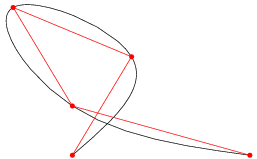
\includegraphics[width=\textwidth]{bilder/kubikSpline}
\end{minipage}

\textbf{Properties}
\begin{liste}
  \item[\textbf{+}] No Runge phenomenon (oscillations at the boundaries)
  \item[\textbf{+}] Polynomials have low degree
  \item[\textbf{+}] Computation effort lower than Newton [Spline: $O(n)$ (due to tridiagonal band matrix),Newton: $O(n^2)$]
  \item[$\mathbf{-}$] "Not embedded" (new measurements mean new polynomial calculation!)
  \item[$\mathbf{-}$] Polynomials must be composed for evaluation (post-processing effort is large)
\end{liste}


\subsection{One-Dimensional Splines}
\subsubsection{Principle}
For each \em patch \em (out of a total of $n$), a polynomial of degree $d$ (usually cubic, $d=3$) is computed.
Conditions $C^k$ ($k=1,\ldots, d-1$) can be defined at the transitions at $x_i$.

\paragraph{Degrees of Freedom}
$n$ patches with 1 polynomial each with $(d+1)$ coefficients each give a total of $n(d+1)$ degrees of freedom.

\paragraph{Conditions}
$n$ patches with start and end $=2n$;
$d-1$ derivatives per inner point $(n-1)(d-1)$ result in a total of $(n(d+1)-(d-1))$ conditions.

\paragraph{Additional Conditions}
When comparing degrees of freedom and conditions, $d-1$ conditions need to be chosen. For the \em natural
spline, \em the second derivatives are set to 0; for \em clamped splines,
\em the first derivatives are specified.


\subsubsection{General Procedure (Cubic Splines)}
The final interpolation has the following form (description of \textbf{one} patch):
$$\boxed{S_i(x) = a_i + b_i(x-x_i) + c_i(x-x_i)^2 + d_i(x-x_i)^3}$$
$$S_i' = b_i + 2c_i(x-x_i)+3d_i(x-x_i)^2$$
$$S_i'' = 2c_i + 6 d_i (x-x_i)$$
Also needed (patch width) $h_i = x_{i+1} - x_i = \Delta x_i$
\begin{enumerate}
  \item $a_i = y_i \qquad (i=0,\ldots n-1)$
  \item For cubic splines, there are $d-1=3-1=2$ additional conditions.\\ 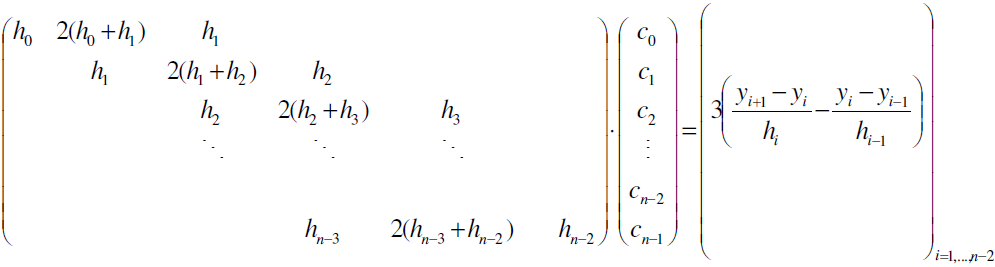
\includegraphics[width=12cm]{./bilder/1d_spline_gleichungssystem}
\newpage
    \begin{itemize}
      \item \textbf{Natural Spline} (Boundary curvature): $y_0''=0=y_n''$ (minimizes the energy norm! ($\min \int |f''(x)|^2 \mathrm{d}x$))
        \begin{enumerate}
          \item $c_0 = c_n = 0$
          \item Solve the system of equations for $c_i$:\\
            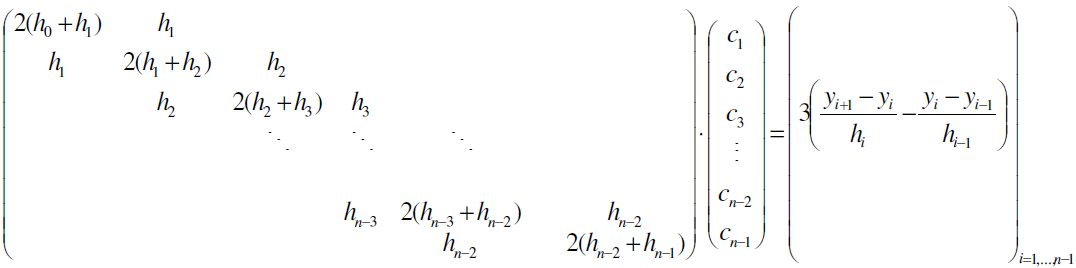
\includegraphics[width=13cm]{./bilder/1d_spline_natural_gleichungssystem}
          %\item $d_{n-1} = -\frac{c_{n-1}}{3h_{n-1}}$
        \end{enumerate}
       \item \textbf{Clamped Spline:}
         \begin{enumerate}
           \item $b_0 = y_0'; b_n=y_n'$
           \item Solve the system of equations for $c_i$:\\
             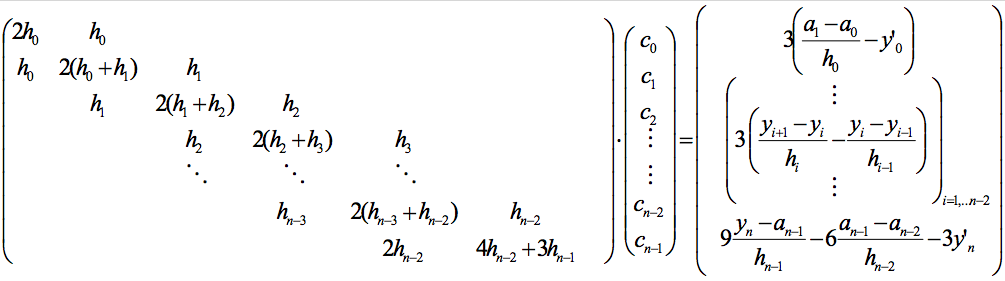
\includegraphics[width=12cm]{./bilder/ClampedSplining}
           %\item $d_{n-1} = \frac{y_n' - b_{n-1} - 2c_{n-1}h_{n-1}}{3h_{n-1}^2}$ (to be calculated at the end)
         \end{enumerate}
    \end{itemize}
  \item $b_{i-1} = \frac{a_i - a_{i-1}}{h_{i-1}} - \frac{2 c_{i-1} + c_i}{3} h_{i-1} \qquad (i=1, \ldots, n-1)$
  \item $b_{n-1} = \frac{y_n - a_{n-1}}{h_{n-1}} - c_{n-1} h_{n-1} - d_{n-1}h_{n-1}^2=\frac{y_n-y_{n-1}}{h_{n-1}}-\frac 23 c_{n-1}h_{n-1}$
  \item $d_{i-1} = \frac{c_i - c_{i-1}}{3 h_{i-1}} \qquad (i=1, \ldots n-1)$
  \item Clamped Spline: $d_{n-1} = \frac{y_n' - b_{n-1} - 2c_{n-1}h_{n-1}}{3h_{n-1}^2}$ \hspace{1cm} Natural Spline: $d_{n-1} = -\frac{c_{n-1}}{3h_{n-1}}$
\end{enumerate}


\paragraph{Further Methods}~\\
In \emph{Hermite cubic splines}, $C^1$ functions are formed from patched cubic polynomials with
prescribed first derivatives.

\emph{Periodic splines} are $C^2$ functions formed from patched cubic polynomials with periodicity ($S'(x_0)=S'(x_n)$ and $S''(x_0)=S''(x_n)$).

\subsubsection{Error Estimation}
For cubic splines with $C^2$, the following error estimate applies ($H = \max h_i \; (i=0, \ldots n-1)$):\\
$| y(x) - S(x) | \leq \max |y^{(4)}(x)| \frac{5}{384} H^4 \qquad
 | y'(x) - S'(x) | \leq \max |y^{(4)}(x)| \frac{1}{24} H^3 \qquad
 | y''(x) - S''(x) | \leq \max |y^{(4)}(x)| \frac{3}{8} H^2$


\newpage
\subsection{Bernstein-Bézier Splines (B-B Splines)}

\begin{minipage}[c]{15.0cm}
	\subsubsection{Bernstein Polynomials}\label{sssec:spline_bernsteinpoly}
    	The Bernstein polynomials are defined in the interval $t\in[0,1]$ as
	    \[B_{i,n}(t) = \binom{n}{i}(1-t)^{n-i} t^i \qquad t \in [0,1]\; i=0,1,\ldots, n\]
	    with $i$: index and  $n$: order of the spline.

      Through an affine transformation into the interval $t \in [a,b]$, we have
	    \[B_{i,n}(u,a,b) =\frac{1}{(b-a)^n}\binom{n}{i}(b-u)^{n-i} (u-a)^i \qquad u \in [a,b]\; i=0,1,\ldots, n\]

      \paragraph{Properties}
      Bernstein polynomials$\ldots$
        \begin{itemize}
          \item form a linear basis for polynomials of order $n$ (they can be used to build any polynomial of order $n$)
          \item have exactly one maximum at $t=\frac in$
          \item have a root at $0$ (order $i$) and at $1$ (order $n-1$)
          \item are symmetric: $B_{i,n}(t) = B_{n-i,n}(1-t)$
          \item are bounded between $t \in [0,1]$ and are restricted to $[0,1]$
          \item sum up to: $\sum \limits_{i=0}^n B_{i,n}(t)=1$
        \end{itemize}

	    $\frac{d}{dt} B_{i,n}(t) = n(B_{i-1,n-1}(t) - B_{i,n-1}(t)) = -n \Delta B_{i-1,n-1}(t)$\\
	    $\frac{d^2}{dt^2} B_{i,n}(t) = n(n-1)(B_{i-2,n-2}(t) -2 B_{i-1,n-2}(t) + B_{i,n-2}(t)) = n(n-1) \Delta^2 B_{i-2,n-2}(t)$\\
	    $\frac{d^k}{dt^k} B_{i,n}(t) = (-1)^k n(n-1)\ldots(n-k+1) \Delta^k B_{i-k,n-k}(t)$
\end{minipage}
\hfill
\begin{minipage}[c]{4cm}
  	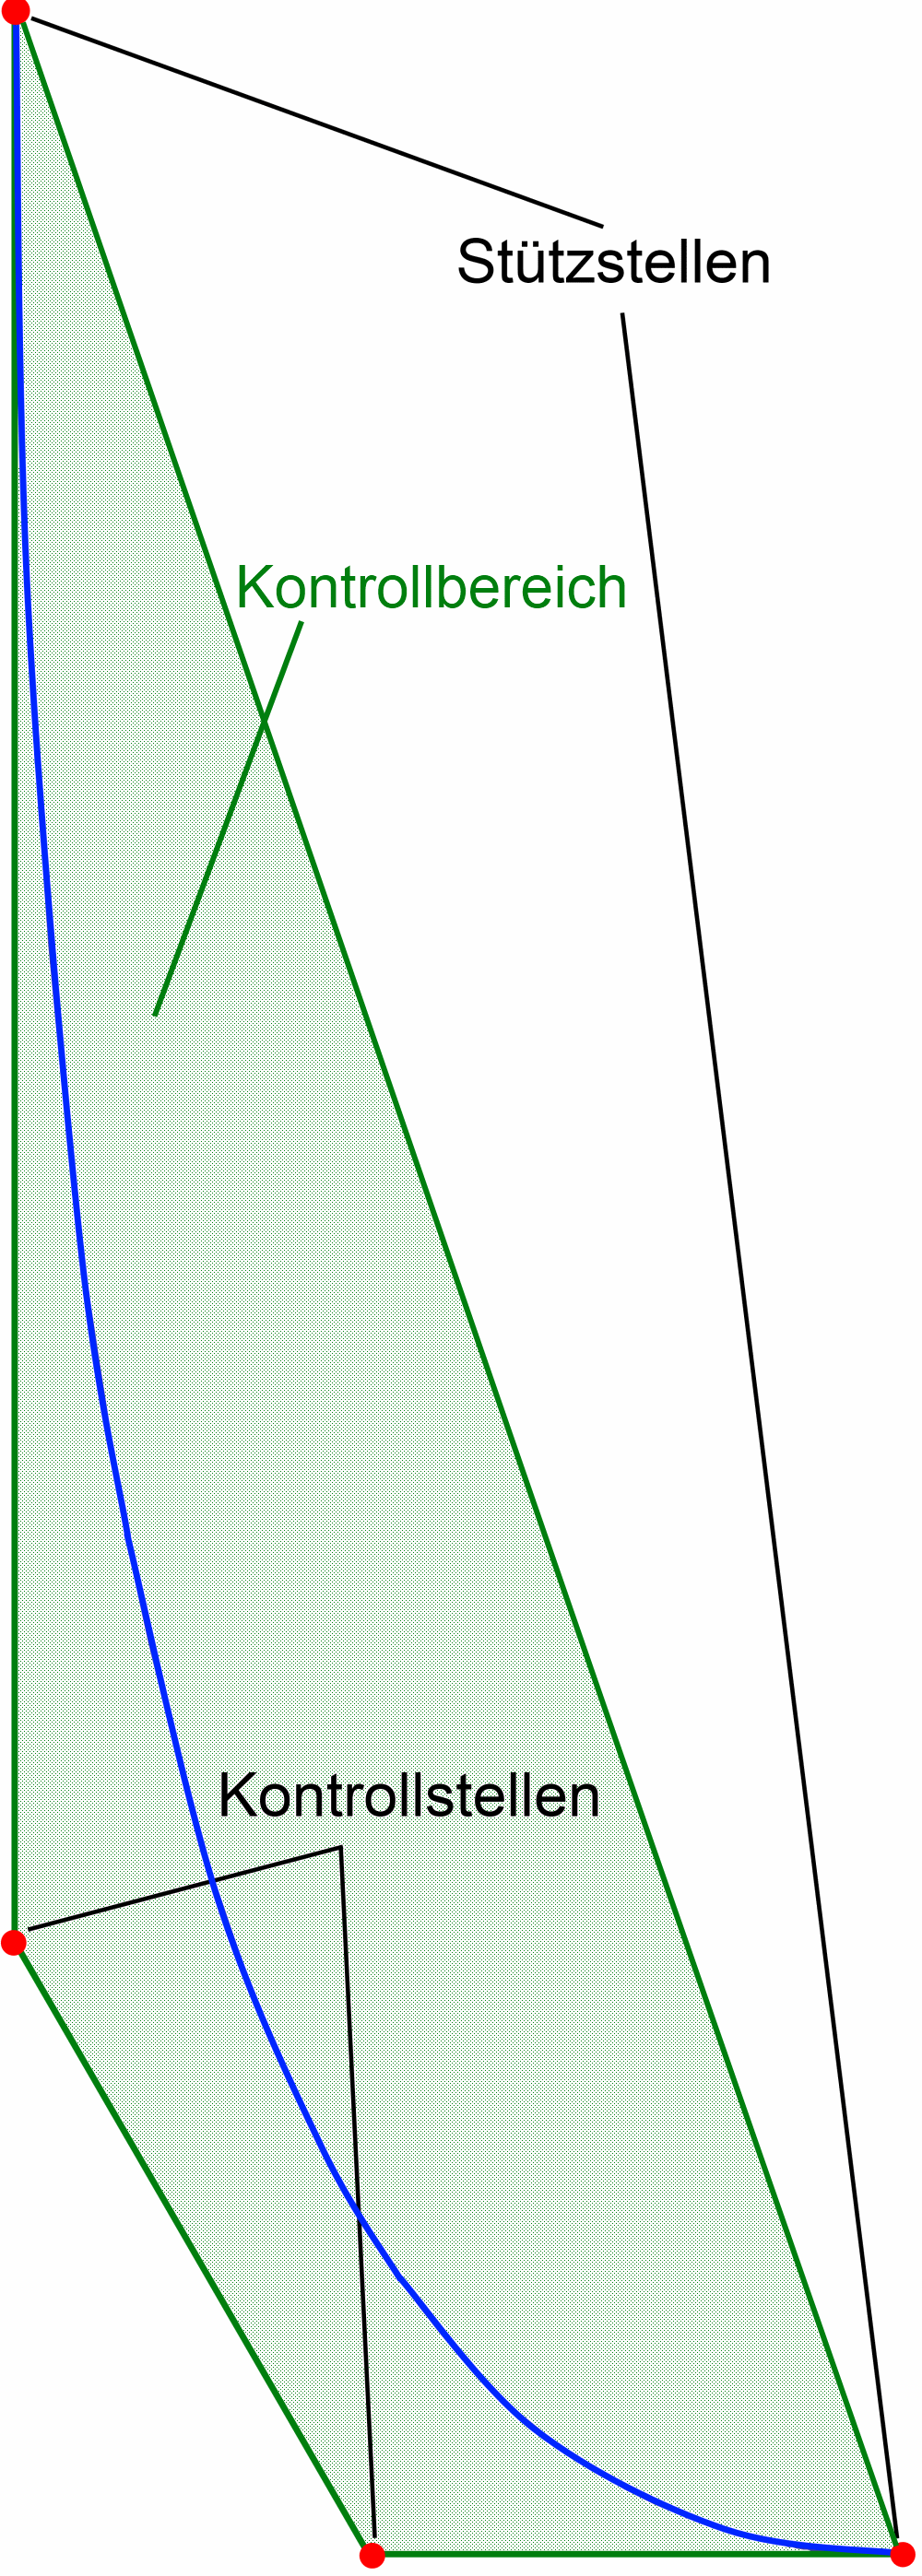
\includegraphics[width=\textwidth]{bilder/bernsteinBezier}
\end{minipage}

\vspace{0.2cm}

\begin{minipage}[c]{5.5cm}
\textbf{Pascal's Triangle}\\

	\scalebox{0.8}{
	\renewcommand{\arraystretch}{1}
	\begin{tabular}{rccccccccc}
		$n=0$:&    &    &    &    &  1\\\noalign{\smallskip\smallskip}
		$n=1$:&    &    &    &  1 &    &  1\\\noalign{\smallskip\smallskip}
		$n=2$:&    &    &  1 &    &  2 &    &  1\\\noalign{\smallskip\smallskip}
		$n=3$:&    &  1 &    &  3 &    &  3 &    &  1\\\noalign{\smallskip\smallskip}
		$n=4$:&  1 &    &  4 &    &  6 &    &  4 &    &  1\\\noalign{\smallskip\smallskip}
	\end{tabular}}
\end{minipage}
\hfill
\begin{minipage}[c]{13.25cm}
\textbf{Bernstein Polynomials} \quad $0\leq t\leq 1$\\

	\scalebox{0.8}{
	\begin{tabular}{lllll}
		$B_{0,0}(t)=1$&&&&\\
		$B_{0,1}(t)=1-t$&$B_{1,1}(t)=t$&&&\\
		$B_{0,2}(t)=(1-t)^2$&$B_{1,2}(t)=2t(1-t)$&$B_{2,2}(t)=t^2$&&\\
		$B_{0,3}(t)=(1-t)^3$&$B_{1,3}(t)=3t(1-t)^2$&$B_{2,3}(t)=3t^2(1-t)$&$B_{3,3}(t)=t^3$&\\
		$B_{0,4}(t)=(1-t)^4$&$B_{1,4}(t)=4t(1-t)^3$&$B_{2,4}(t)=6t^2(1-t)^2$&$B_{3,4}(t)=4t^3(1-t)$&$B_{4,4}(t)=t^4$\\
	\end{tabular}}
\renewcommand{\arraystretch}{1.5}
\end{minipage}


\subsubsection{Simple Bézier Curves}
A Bézier curve is defined by control points ($\vec{P}_0, \vec{P}_1, \ldots \vec{P}_n\,(n \geq 2)$
in $R^d$) and the Bernstein polynomials:
$$\vec{r}(t) = \sum \limits_{i=0}^{n} \vec{P}_i B_{i,n}(t) \quad t \in [0,1]$$
\paragraph{Properties}
\begin{itemize}
  \item Bézier curves always lie within the convex hull of the control points.
  \item \begin{tabular}{ll}
            $\vec{r}(0) = \vec{P}_0$ & $\vec{r}(1) = \vec{P}_n$ \\
            $\vec{r}\,'(0) = n(\vec{P}_1-\vec{P}_0)$ & $\vec{r}\,'(1) = n(\vec{P}_n-\vec{P}_{n-1})$ \\
            $\vec{r}\,''(0) = n(n-1)(\vec{P}_2 - 2\vec{P}_1 + \vec{P}_0)$ & $\vec{r}\,''(1) = n(n-1)(\vec{P}_n - 2\vec{P}_{n-1} + \vec{P}_{n-2})$ \\
        \end{tabular}
  \item If $C^k$ continuity is demanded at a point, $k$ equations or $k$ control points per point are necessary.
\end{itemize}


\begin{minipage}{13.5cm}
\subsubsection{Casteljau Recurrence}
The Casteljau recurrence is a similar idea to Neville-Aitken.
It allows a point on a Bézier curve to be calculated as a linear combination of two points from Bézier curves of lower order.
\[
    \vec{r}_{\vec{P_0},\vec{P_1},\ldots,\vec{P_n}}(t) = (1-t)\cdot\vec{r}_{\vec{P_0},\vec{P_1},\ldots,\vec{P_{n-1}}}(t) + t \cdot \vec{r}_{\vec{P_1},\vec{P_2},\ldots,\vec{P_n}}(t) \qquad t \in [0,1]
\]


\subsubsection{Composite Bézier Curves}
The composite (simple) Bézier curves should satisfy the known conditions ($C^k$).
These are the equations to the point $Q_0$ with control points $Q_{1,\ldots,m-1}$ after $Q_0$, as well as
the control points $P_{1,\ldots,n-1}$ before $Q_0$.
\end{minipage}
\begin{minipage}{5.5cm}
  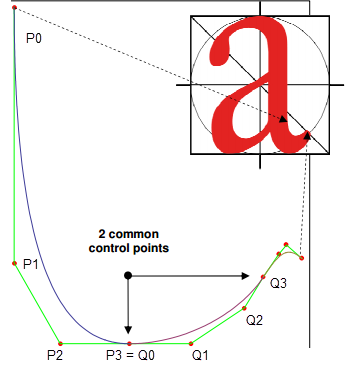
\includegraphics[width=5.5cm]{./bilder/composite_bezier.png}
  Here, $m=n=3$
\end{minipage}

  \begin{align*}
      &C^0: \qquad && &&\boxed{\vec{P_n} = \vec{Q_0}} \\
      &C^1: && \vec{r}\,'_P(1) = &&\boxed{n(\vec{P}_n-\vec{P}_{n-1}) = m(\vec{Q}_1-\vec{Q_0})} && = \vec{r}\,'_Q(0) \\
      &C^2: && \vec{r}\,''_P(1) = &&\boxed{n(n-1)(\vec{P}_n - 2\vec{P}_{n-1} + \vec{P}_{n-2}) =
    m(m-1)(\vec{Q}_2 - 2\vec{Q_1} + \vec{Q_0})} && = \vec{r}\,''_Q(0) \\
      &C^k: && \vec{r}_P^{\,(k)}(1) = && \boxed{n(n-1)\dots(n-k+1)(\Delta^k\vec{P}_{n-k}) =
      m(m-1)\dots(m-k+1)(\Delta^k\vec{Q}_0)} &&= \vec{r}_Q^{\,(k)}(0)
  \end{align*}

  where $m$ is the degree of $\vec{r}_Q$, and $n$ is the degree of $\vec{r}_P$.


\subsubsection{Composite Bézier Curves with $P_{i,j}$}
When $\vec{r_j}(t) = \sum \limits_{i=0}^{n} \vec{P}_{i,j} B_{i,n}(t) \quad t \in [0,1]$ is defined with the fixed points $Q_j$ (degree: $n$), the following formulas are obtained:

  \begin{align*}
      &C^0: \qquad && &&\boxed{\vec{P}_{n,j-1} = \vec{P_{0,j}} = \vec{Q_j}} \\
      &C^1: && \vec{r}\,'_{j-1}(1) = &&\boxed{\vec{Q}_{j}-\vec{P}_{{n-1,j-1}} = \vec{P}_{1,j}-\vec{Q}_j} && = \vec{r}\,'_j(0) \\
      &C^2: && \vec{r}\,''_{j-1}(1) = &&\boxed{\vec{Q}_{j} - 2\vec{P}_{n-1,j-1} + \vec{P}_{n-2,j-1} =
    \vec{P}_{2,j} - 2\vec{P}_{1,j} + \vec{Q_j}} && = \vec{r}\,''_j(0) \\
      &C^k: && \vec{r}_{j-1}^{\,(k)}(1) = && \boxed{\Delta^k\vec{P}_{n-k,j-1} = \Delta^k\vec{P}_{0,j}} &&= \vec{r}_j^{\,(k)}(0)
  \end{align*}

\subsubsection{Bézier Surfaces as Tensor Splines}
Bézier surfaces are formed in the same way as Bézier curves, using a tensor product of Bernstein polynomials.
A surface in the interval $[0,1]\times[0,1]$ is formed by
\[
    \vec{z}(s,t) = \sum\limits_{i=0}^n\sum\limits_{j=0}^m \vec{P}_{ij} B_{in}(s) B_{jm}(t) \qquad s,t\in[0,1]
\]

Details and Formulas see Skript p. 19 -- 23.

\subsubsection{Comparison of Bézier and Newton Interpolation with Equally Distributed Arguments on the X-Axis}
  From the Bézier perspective:
  \begin{itemize}
    \item[+] Small error, no oscillation, no Runge phenomenon (with a low degree, e.g., 3)
    \item[+] $O(n)$ (linear computation effort)
    \item[-] Not embedded (new data requires recalculation of the interpolation)
    \item[-] Post-processing (graphics, integration, derivatives) is more complex, as each curve segment must be considered individually.
  \end{itemize}
